\documentclass[]{book}
\usepackage{lmodern}
\usepackage{amssymb,amsmath}
\usepackage{ifxetex,ifluatex}
\usepackage{fixltx2e} % provides \textsubscript
\ifnum 0\ifxetex 1\fi\ifluatex 1\fi=0 % if pdftex
  \usepackage[T1]{fontenc}
  \usepackage[utf8]{inputenc}
\else % if luatex or xelatex
  \ifxetex
    \usepackage{mathspec}
  \else
    \usepackage{fontspec}
  \fi
  \defaultfontfeatures{Ligatures=TeX,Scale=MatchLowercase}
\fi
% use upquote if available, for straight quotes in verbatim environments
\IfFileExists{upquote.sty}{\usepackage{upquote}}{}
% use microtype if available
\IfFileExists{microtype.sty}{%
\usepackage{microtype}
\UseMicrotypeSet[protrusion]{basicmath} % disable protrusion for tt fonts
}{}
\usepackage{hyperref}
\hypersetup{unicode=true,
            pdftitle={A minimal quantitative RNAseq pipeline},
            pdfauthor={Dan MacLean},
            pdfborder={0 0 0},
            breaklinks=true}
\urlstyle{same}  % don't use monospace font for urls
\usepackage{natbib}
\bibliographystyle{apalike}
\usepackage{color}
\usepackage{fancyvrb}
\newcommand{\VerbBar}{|}
\newcommand{\VERB}{\Verb[commandchars=\\\{\}]}
\DefineVerbatimEnvironment{Highlighting}{Verbatim}{commandchars=\\\{\}}
% Add ',fontsize=\small' for more characters per line
\usepackage{framed}
\definecolor{shadecolor}{RGB}{248,248,248}
\newenvironment{Shaded}{\begin{snugshade}}{\end{snugshade}}
\newcommand{\AlertTok}[1]{\textcolor[rgb]{0.94,0.16,0.16}{#1}}
\newcommand{\AnnotationTok}[1]{\textcolor[rgb]{0.56,0.35,0.01}{\textbf{\textit{#1}}}}
\newcommand{\AttributeTok}[1]{\textcolor[rgb]{0.77,0.63,0.00}{#1}}
\newcommand{\BaseNTok}[1]{\textcolor[rgb]{0.00,0.00,0.81}{#1}}
\newcommand{\BuiltInTok}[1]{#1}
\newcommand{\CharTok}[1]{\textcolor[rgb]{0.31,0.60,0.02}{#1}}
\newcommand{\CommentTok}[1]{\textcolor[rgb]{0.56,0.35,0.01}{\textit{#1}}}
\newcommand{\CommentVarTok}[1]{\textcolor[rgb]{0.56,0.35,0.01}{\textbf{\textit{#1}}}}
\newcommand{\ConstantTok}[1]{\textcolor[rgb]{0.00,0.00,0.00}{#1}}
\newcommand{\ControlFlowTok}[1]{\textcolor[rgb]{0.13,0.29,0.53}{\textbf{#1}}}
\newcommand{\DataTypeTok}[1]{\textcolor[rgb]{0.13,0.29,0.53}{#1}}
\newcommand{\DecValTok}[1]{\textcolor[rgb]{0.00,0.00,0.81}{#1}}
\newcommand{\DocumentationTok}[1]{\textcolor[rgb]{0.56,0.35,0.01}{\textbf{\textit{#1}}}}
\newcommand{\ErrorTok}[1]{\textcolor[rgb]{0.64,0.00,0.00}{\textbf{#1}}}
\newcommand{\ExtensionTok}[1]{#1}
\newcommand{\FloatTok}[1]{\textcolor[rgb]{0.00,0.00,0.81}{#1}}
\newcommand{\FunctionTok}[1]{\textcolor[rgb]{0.00,0.00,0.00}{#1}}
\newcommand{\ImportTok}[1]{#1}
\newcommand{\InformationTok}[1]{\textcolor[rgb]{0.56,0.35,0.01}{\textbf{\textit{#1}}}}
\newcommand{\KeywordTok}[1]{\textcolor[rgb]{0.13,0.29,0.53}{\textbf{#1}}}
\newcommand{\NormalTok}[1]{#1}
\newcommand{\OperatorTok}[1]{\textcolor[rgb]{0.81,0.36,0.00}{\textbf{#1}}}
\newcommand{\OtherTok}[1]{\textcolor[rgb]{0.56,0.35,0.01}{#1}}
\newcommand{\PreprocessorTok}[1]{\textcolor[rgb]{0.56,0.35,0.01}{\textit{#1}}}
\newcommand{\RegionMarkerTok}[1]{#1}
\newcommand{\SpecialCharTok}[1]{\textcolor[rgb]{0.00,0.00,0.00}{#1}}
\newcommand{\SpecialStringTok}[1]{\textcolor[rgb]{0.31,0.60,0.02}{#1}}
\newcommand{\StringTok}[1]{\textcolor[rgb]{0.31,0.60,0.02}{#1}}
\newcommand{\VariableTok}[1]{\textcolor[rgb]{0.00,0.00,0.00}{#1}}
\newcommand{\VerbatimStringTok}[1]{\textcolor[rgb]{0.31,0.60,0.02}{#1}}
\newcommand{\WarningTok}[1]{\textcolor[rgb]{0.56,0.35,0.01}{\textbf{\textit{#1}}}}
\usepackage{longtable,booktabs}
\usepackage{graphicx,grffile}
\makeatletter
\def\maxwidth{\ifdim\Gin@nat@width>\linewidth\linewidth\else\Gin@nat@width\fi}
\def\maxheight{\ifdim\Gin@nat@height>\textheight\textheight\else\Gin@nat@height\fi}
\makeatother
% Scale images if necessary, so that they will not overflow the page
% margins by default, and it is still possible to overwrite the defaults
% using explicit options in \includegraphics[width, height, ...]{}
\setkeys{Gin}{width=\maxwidth,height=\maxheight,keepaspectratio}
\IfFileExists{parskip.sty}{%
\usepackage{parskip}
}{% else
\setlength{\parindent}{0pt}
\setlength{\parskip}{6pt plus 2pt minus 1pt}
}
\setlength{\emergencystretch}{3em}  % prevent overfull lines
\providecommand{\tightlist}{%
  \setlength{\itemsep}{0pt}\setlength{\parskip}{0pt}}
\setcounter{secnumdepth}{5}
% Redefines (sub)paragraphs to behave more like sections
\ifx\paragraph\undefined\else
\let\oldparagraph\paragraph
\renewcommand{\paragraph}[1]{\oldparagraph{#1}\mbox{}}
\fi
\ifx\subparagraph\undefined\else
\let\oldsubparagraph\subparagraph
\renewcommand{\subparagraph}[1]{\oldsubparagraph{#1}\mbox{}}
\fi

%%% Use protect on footnotes to avoid problems with footnotes in titles
\let\rmarkdownfootnote\footnote%
\def\footnote{\protect\rmarkdownfootnote}

%%% Change title format to be more compact
\usepackage{titling}

% Create subtitle command for use in maketitle
\providecommand{\subtitle}[1]{
  \posttitle{
    \begin{center}\large#1\end{center}
    }
}

\setlength{\droptitle}{-2em}

  \title{A minimal quantitative RNAseq pipeline}
    \pretitle{\vspace{\droptitle}\centering\huge}
  \posttitle{\par}
    \author{Dan MacLean}
    \preauthor{\centering\large\emph}
  \postauthor{\par}
      \predate{\centering\large\emph}
  \postdate{\par}
    \date{2020-01-24}

\usepackage{booktabs}
\usepackage{amsthm}
\makeatletter
\def\thm@space@setup{%
  \thm@preskip=8pt plus 2pt minus 4pt
  \thm@postskip=\thm@preskip
}
\makeatother

\begin{document}
\maketitle

{
\setcounter{tocdepth}{1}
\tableofcontents
}
\hypertarget{about-this-course}{%
\chapter{About this course}\label{about-this-course}}

In this short course we'll look at a method for getting quantitative estimates of gene expression from RNAseq data. The course assumes that you will already have performed a read alignment so is \emph{not} a `read to results' course. The course is very brief and will show you how to use a perform a common pipeline centered around \texttt{DESeq} in \texttt{R} and \texttt{RStudio}

I acknowledge that there are lots of other programs and methods - this course is \emph{not} meant to be comprehensive, it is meant to get you being productive. Seek out further advice if you need to run other programs or systems. Do be encouraged though, lots of what you learn here will be applicable to other pipelines for the same job (they all run in a similar manner with similar objects) so this is a good place to start.

The course is intended to run on your `local' machine, that is to say, your laptop or desktop computer. In general these machines will be powerful enough for most datasets though the pipeline we will learn can be easily adapted for a high performance computing environment if you need greater computational power.

\hypertarget{prerequisites}{%
\section{Prerequisites}\label{prerequisites}}

This course assumes that you are a little familiar with the basics of running R and R commands from the R console. You'll need to know the basics of typing in commands and getting output, not much more.

\hypertarget{r-and-rstudio}{%
\subsection{R and RStudio}\label{r-and-rstudio}}

\hypertarget{installing-r}{%
\subsubsection{Installing R}\label{installing-r}}

Follow this link and install the right version for your operating system \url{https://www.stats.bris.ac.uk/R/}

\hypertarget{installing-rstudio}{%
\subsubsection{Installing RStudio}\label{installing-rstudio}}

Follow this link and install the right version for your operating system \url{https://www.rstudio.com/products/rstudio/download/}

\hypertarget{installing-r-packages-in-rstudio.}{%
\subsubsection{Installing R packages in RStudio.}\label{installing-r-packages-in-rstudio.}}

You'll need the following R packages:

\begin{enumerate}
\def\labelenumi{\arabic{enumi}.}
\tightlist
\item
  devtools
\item
  atacR
\item
  DESeq
\end{enumerate}

For simplicity, install them in that order.

To install \texttt{devtools}:

Start RStudio and use the \texttt{Packages} tab in lower right panel. Click the install button (top left of the panel) and enter the package name \texttt{devtools}, then click install as in this picture

\begin{figure}
\centering
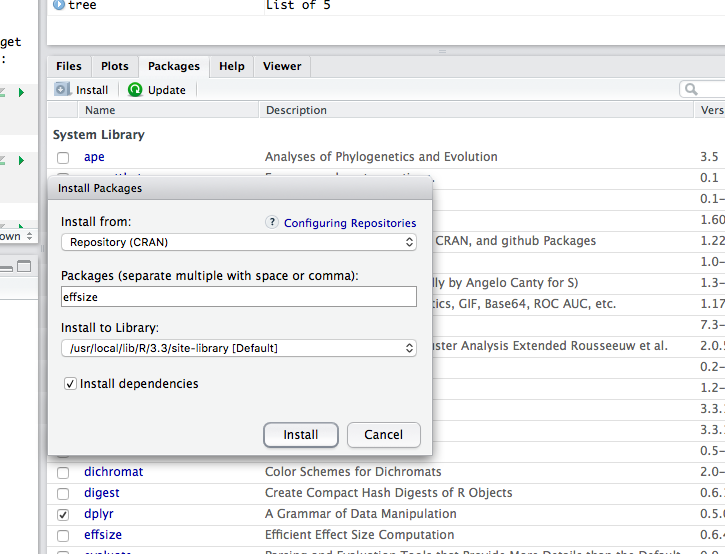
\includegraphics{fig/package_install.png}
\caption{Installing Packages}
\end{figure}

To install \texttt{atacR}:

Type the following into the RStudio console, \texttt{devtools::install\_github("TeamMacLean/atacr")}

To install \texttt{DESeq}:

Type the following into the RStudio console, \texttt{BiocManager::install("DESeq")}

Now you are done! Everything is installed ready for you to work with. Next we need to get the sample data

\hypertarget{sample-reference-genome-and-reads}{%
\subsection{Sample reference genome and reads}\label{sample-reference-genome-and-reads}}

You'll need this zip file of data: \href{https://github.com/TeamMacLean/basic_alignment/raw/master/sample_data/sample_data.zip}{sample\_data.zip} which contains a reference genome and a set of paired end reads. Download it, extract the files and put them into a folder on your machine. I suggest something like \texttt{Desktop/align\_tut}. This will be the directory we'll work from in the rest of the course.

That's all you need to do the lesson. If you have any problems getting this going, then ask someone in the Bioinformatics Team and we'll help.

\hypertarget{intro}{%
\chapter{Counting Aligned Reads in Genomic Regions}\label{intro}}

\hypertarget{about-this-chapter}{%
\section{About this chapter}\label{about-this-chapter}}

\begin{enumerate}
\def\labelenumi{\arabic{enumi}.}
\tightlist
\item
  Questions
\end{enumerate}

\begin{itemize}
\tightlist
\item
  How do I calculate counts of reads at genes from my alignments?
\end{itemize}

\begin{enumerate}
\def\labelenumi{\arabic{enumi}.}
\setcounter{enumi}{1}
\tightlist
\item
  Objectives
\end{enumerate}

\begin{itemize}
\tightlist
\item
  Understand the basis for the gene region and read counting technique
\item
  Understand what the count matrix represents
\item
  Use the \texttt{make\_counts()} function to make a count matrix
\end{itemize}

\begin{enumerate}
\def\labelenumi{\arabic{enumi}.}
\setcounter{enumi}{2}
\tightlist
\item
  Keypoints
\end{enumerate}

\begin{itemize}
\tightlist
\item
  Gene regions are designated by coordinates in GFF files
\item
  A count matrix is a table-like object of reads that are found in a given genomic region
\item
  The count matrix is the main object in a DESeq analysis
\end{itemize}

In this chapter we'll look at the fundamentals of read counting from a BAM file of aligned reads.

\hypertarget{counting-the-number-of-reads-that-have-aligned-to-gene-regions}{%
\section{Counting the number of reads that have aligned to gene regions}\label{counting-the-number-of-reads-that-have-aligned-to-gene-regions}}

The basis of quantitative RNAseq is working out how many of our sequence reads have aligned to each gene. In broad terms this is done by taking the genomic coordinates of all the aligned reads (the start and end positions of the read's alignment on the reference genome) and cross-referencing them with the positions of the genes from a gene file. The resulting table is called a count matrix. See the figure below for a representation.

\begin{figure}
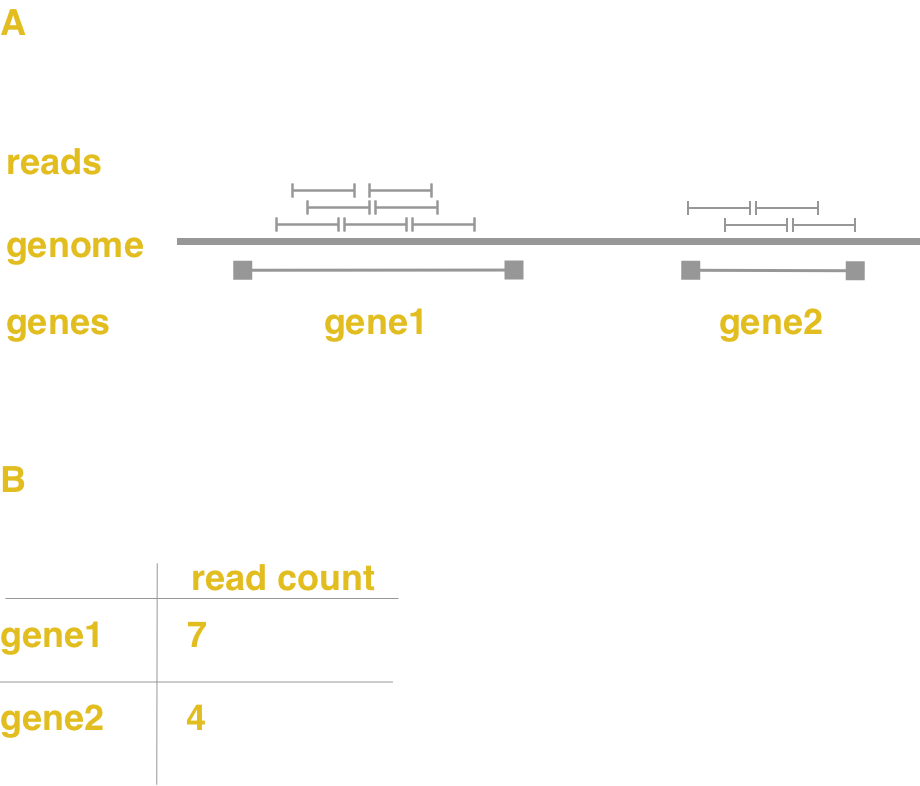
\includegraphics[width=12.78in]{fig/align} \caption{A) Graphic of read alignment and gene position showing reads within genes. B) The equivalent count matrix that comes from this alignment}\label{fig:unnamed-chunk-1}
\end{figure}

It is our aim in this section to create a count matrix from BAM files.

\hypertarget{atacr}{%
\subsection{atacR}\label{atacr}}

\texttt{atacR} was initially designed to help with the analysis of ATAC-Cap-seq data, a quite differen sort of data to RNAseq, but as with many bioinformatics pipelines, the first steps are quite common so we can make use of the neat way \texttt{atacR} handles the count matrix creation in the helpful function \texttt{make\_counts()}

\hypertarget{preparing-the-input}{%
\section{Preparing the input}\label{preparing-the-input}}

We needs three things to work: the BAM files, a GFF file and a file of sample information.

\hypertarget{the-gff-file}{%
\subsection{The GFF file}\label{the-gff-file}}

GFF files are one way among many of describing the positions of genes on a genome. Here's a quick look at one.

\begin{verbatim}
chr123  .  gene  1300  1500  .  +  .  ID=gene1
chr123  .  gene  1050  1500  .  +  .  ID=gene2
\end{verbatim}

As you can see, it's a simple file with a gene represented on each line, by its chromosome (\texttt{chr123}), its start and end and its strand. The best thing about GFF files is that usually we can just download them from the relevant genome website. They tend to be freely available.

\hypertarget{the-sample-information-file}{%
\subsection{The Sample Information file}\label{the-sample-information-file}}

This file is a really simple file that references the BAM file of the alignment with the sample and replicate information. It has three columns: \texttt{sample\_name}, \texttt{bam\_file\_path} and \texttt{treatment}.
Here is an example.

\begin{verbatim}
## Parsed with column specification:
## cols(
##   treatment = col_character(),
##   sample_name = col_character(),
##   bam_file_path = col_character()
## )
\end{verbatim}

\begin{tabular}{l|l|l}
\hline
treatment & sample\_name & bam\_file\_path\\
\hline
control & control\_rep1 & sample\_data/control1/alignedSorted.bam\\
\hline
control & control\_rep2 & sample\_data/control2/alignedSorted.bam\\
\hline
control & control\_rep3 & sample\_data/control3/alignedSorted.bam\\
\hline
treatment & treatment\_rep1 & sample\_data/treatment1/alignedSorted.bam\\
\hline
treatment & treatment\_rep2 & sample\_data/treatment2/alignedSorted.bam\\
\hline
treatment & treatment\_rep3 & sample\_data/treatment3/alignedSorted.bam\\
\hline
\end{tabular}

The \texttt{sample\_name} column describes the treatment and replicate performed, the \texttt{bam\_file\_path} describes the place in which the BAM file for that sample is saved and \texttt{treatment} is the general name for the treatment that was used; this column is usually not unique when you have replicates.

\hypertarget{the-bam-files}{%
\subsection{The BAM files}\label{the-bam-files}}

The BAM files all come from a previously done alignment. The sample information file describes the place where they are kept and the sample they represent.

\hypertarget{sample-files-for-this-chapter}{%
\subsection{Sample files for this chapter}\label{sample-files-for-this-chapter}}

All the files are provided for you in the sample data you downloaded as \texttt{50\_genes.gff} and \texttt{sample\_information.csv} and in the folders containing BAM files. Feel free to examine them and look at how they relate to each other.

Once we have these files prepared, we can go on to use the \texttt{atacR} package to make the count matrix.

\hypertarget{running-make_counts}{%
\section{\texorpdfstring{Running \texttt{make\_counts()}}{Running make\_counts()}}\label{running-make_counts}}

First we must load in \texttt{atacR}. Type the following into the R console.

\begin{Shaded}
\begin{Highlighting}[]
\KeywordTok{library}\NormalTok{(atacr)}
\end{Highlighting}
\end{Shaded}

Now we can do the counting with \texttt{make\_counts()}. Here's how to do it. Remember to properly describe the path to the files. The paths given here are correct if the files are in a folder called \texttt{sample\_data} in the current working directory.

\begin{Shaded}
\begin{Highlighting}[]
\NormalTok{count_information <-}\StringTok{ }\KeywordTok{make_counts}\NormalTok{(}\StringTok{"sample_data/50_genes.gff"}\NormalTok{,}
                                 \StringTok{"sample_data/sample_information.csv"}\NormalTok{,}
                                 \DataTypeTok{is_rnaseq =} \OtherTok{TRUE}
\NormalTok{                                 )}
\end{Highlighting}
\end{Shaded}

The function should run and give no output. Note that it is important to set \texttt{is\_rnaseq} to \texttt{TRUE} to tell the function to count appropriately. The results are saved in the \texttt{count\_information} object.

\hypertarget{summaries-and-diagnostic-plots}{%
\section{Summaries and Diagnostic plots}\label{summaries-and-diagnostic-plots}}

With the counts computed we can do some diagnosis on the quality of the experiment.

We can see summary information with the \texttt{summary()} function

\begin{Shaded}
\begin{Highlighting}[]
\KeywordTok{summary}\NormalTok{(count_information)}
\end{Highlighting}
\end{Shaded}

\begin{verbatim}
## ATAC-seq experiment of 2 treatments in 6 samples
##  Treatments: control,treatment 
##  Samples: control_rep1,control_rep2,control_rep3,treatment_rep1,treatment_rep2,treatment_rep3 
##  Bait regions used: 50 
##  Total Windows: 99 
##  
##  On/Off target read counts:
##            sample off_target on_target percent_on_target
## 1   control_rep1          0     57733               100
## 2   control_rep2          0     66155               100
## 3   control_rep3          0     66122               100
## 4 treatment_rep1          0    100547               100
## 5 treatment_rep2          0    120325               100
## 6 treatment_rep3          0    107611               100 
##  Quantiles: 
##  $bait_windows
##     control_rep1 control_rep2 control_rep3 treatment_rep1 treatment_rep2
## 1%        149.48       294.60       241.12         228.70         102.98
## 5%        386.35       437.75       340.50         328.30         193.90
## 95%      2335.20      2438.20      2927.10        4445.90        6940.20
## 99%      3054.18      2752.19      3291.34        5234.33        9423.95
##     treatment_rep3
## 1%          116.50
## 5%          324.00
## 95%        4438.75
## 99%        6948.15
## 
## $non_bait_windows
##     control_rep1 control_rep2 control_rep3 treatment_rep1 treatment_rep2
## 1%             0            0            0              0              0
## 5%             0            0            0              0              0
## 95%            0            0            0              0              0
## 99%            0            0            0              0              0
##     treatment_rep3
## 1%               0
## 5%               0
## 95%              0
## 99%              0
##  
##  Read depths:
##            sample off_target on_target
## 1   control_rep1          0   1154.66
## 2   control_rep2          0   1323.10
## 3   control_rep3          0   1322.44
## 4 treatment_rep1          0   2010.94
## 5 treatment_rep2          0   2406.50
## 6 treatment_rep3          0   2152.22
\end{verbatim}

It is long, but actually quite helpful. The first thing to note is that the words relate to ATAC-Cap-Seq, but in our context `bait regions' just mean gene regions and non-bait just means intergenic regions. The `on\_targets' are read hits to genes, the `off\_targets' are read hits to intergenic regions.

We can see that all the reads have hit in gene regions; that the read depth distribution of genes from the quantiles section give depths in the 1000 - 2000 range. This sort of summary is helpful when you're trying to work out whether the RNAseq is useful, lots of reads `off target' is bad, as is low depth.

\hypertarget{gene-count-plots}{%
\subsection{Gene Count Plots}\label{gene-count-plots}}

We can see the distribution of depths over genes as a plot using the \texttt{plot\_counts()} function

\begin{Shaded}
\begin{Highlighting}[]
\KeywordTok{plot_counts}\NormalTok{(count_information, }\DataTypeTok{log10 =} \OtherTok{FALSE}\NormalTok{)}
\end{Highlighting}
\end{Shaded}

\begin{verbatim}
## Picking joint bandwidth of 488
\end{verbatim}

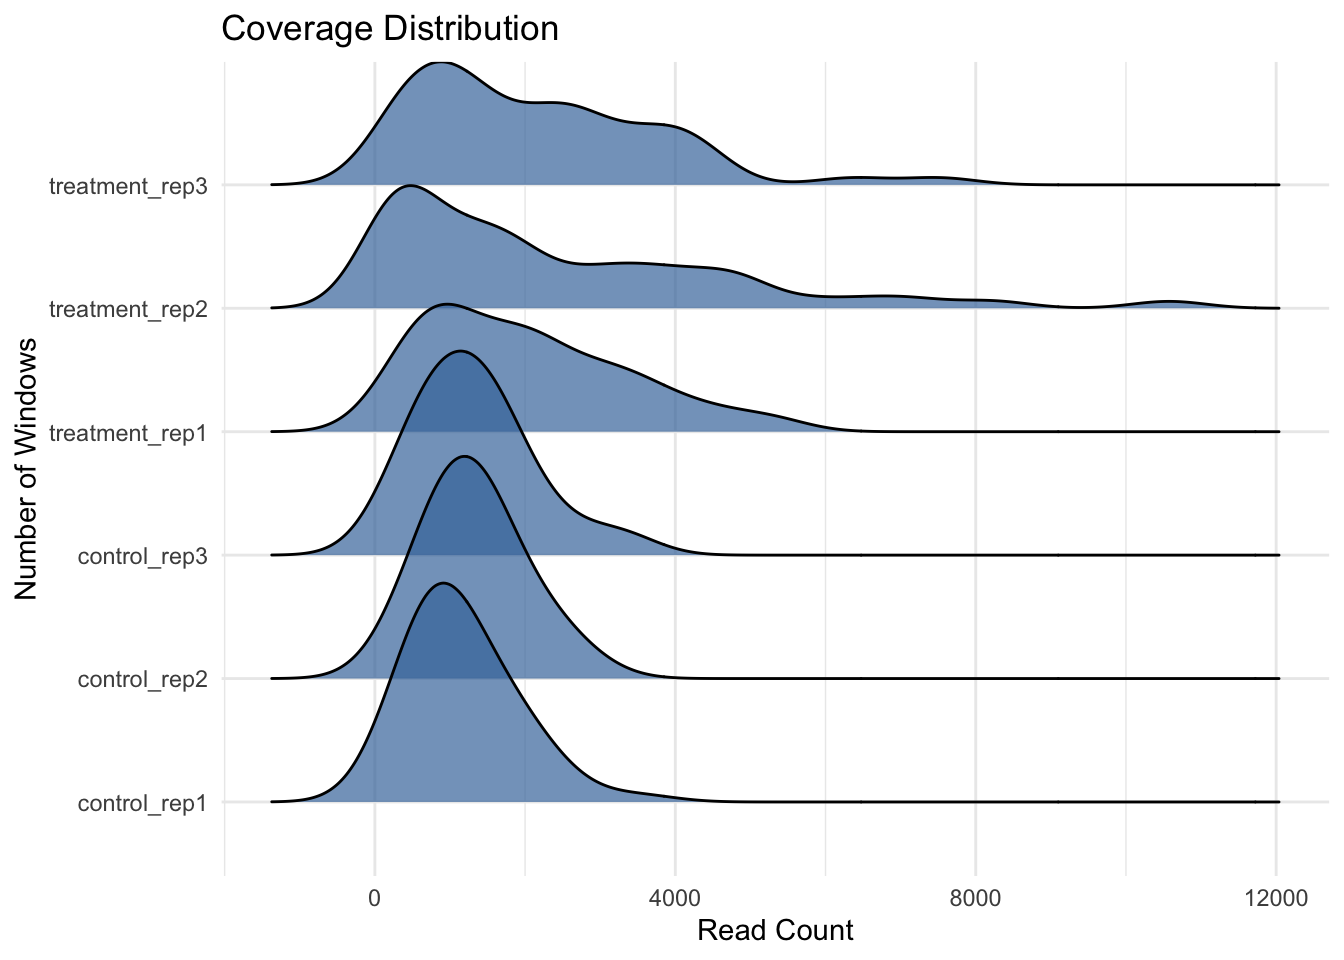
\includegraphics{01-counting_genes_files/figure-latex/unnamed-chunk-6-1.pdf}

We can see that the mean count per gene (windows in \texttt{atacR}) is about 1000. The distributions in the treatment are bit more skewed than the controls.

\hypertarget{comparing-samples-with-pca}{%
\subsection{Comparing Samples with PCA}\label{comparing-samples-with-pca}}

It is common to examine the similarity of the samples to each other before moving on with analysis, ideally the similar samples will cluster together.

With \texttt{atacR} it is easy to perform a quick PCA analysis.

\begin{Shaded}
\begin{Highlighting}[]
\KeywordTok{sample_pca_plot}\NormalTok{(count_information)}
\end{Highlighting}
\end{Shaded}

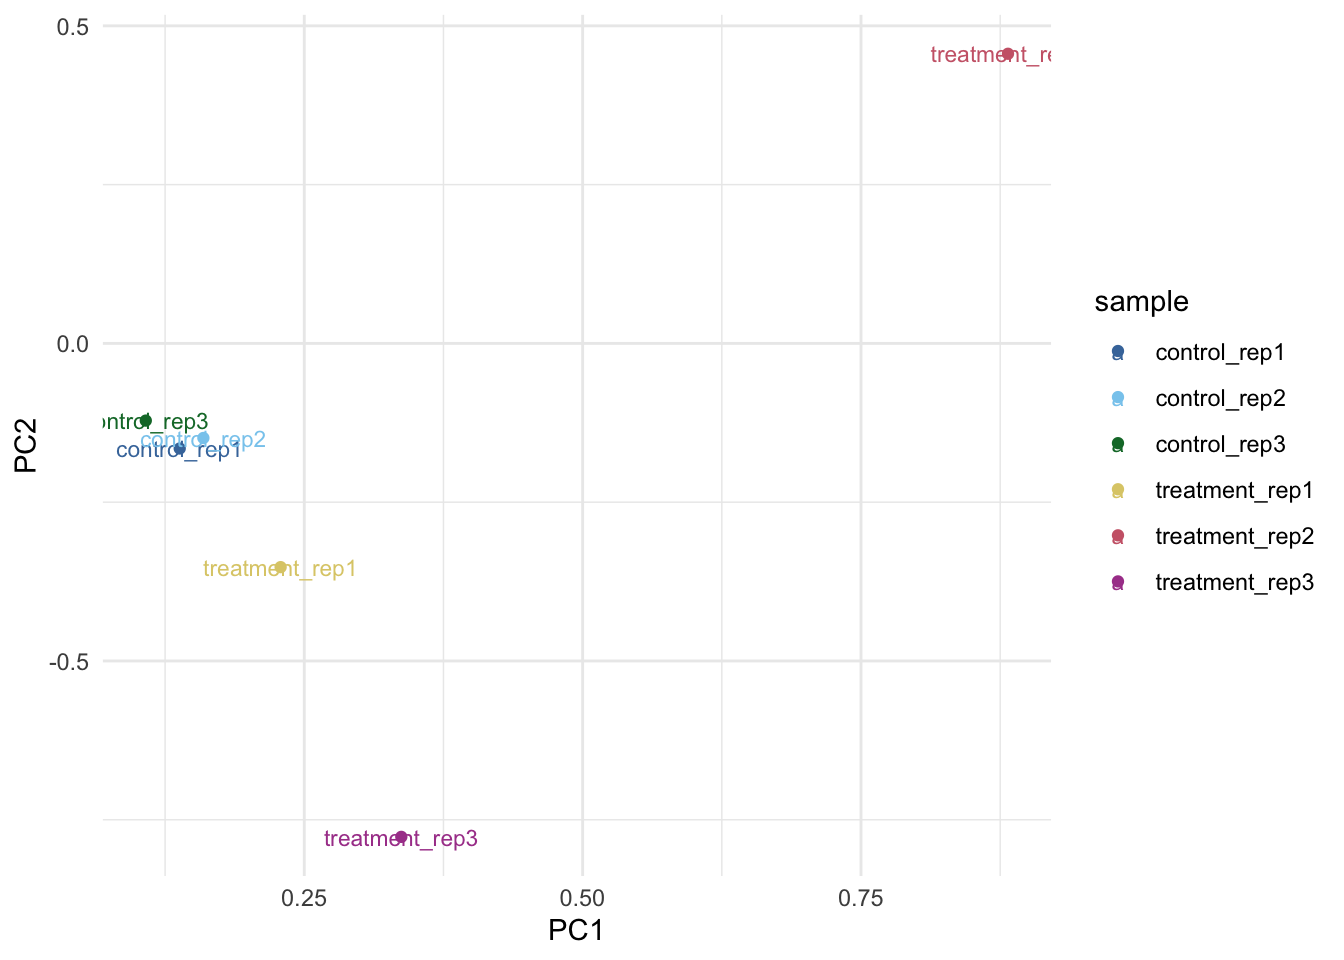
\includegraphics{01-counting_genes_files/figure-latex/unnamed-chunk-7-1.pdf}

Here we can see that the control samples all cluster together, but the treatment samples are a bit more variable. We might want to normalise these counts later as a consequence.

\hypertarget{extracting-and-saving-the-count-matrix}{%
\section{Extracting and saving the count matrix}\label{extracting-and-saving-the-count-matrix}}

We now want to extract out the actual counts hiding inside the \texttt{count\_information} object, we can do this with the \texttt{assay()} extractor function from the \texttt{Summarized\ Experiment} package.

\begin{Shaded}
\begin{Highlighting}[]
\KeywordTok{library}\NormalTok{(SummarizedExperiment)}
\NormalTok{raw_counts <-}\StringTok{ }\KeywordTok{assay}\NormalTok{(count_information}\OperatorTok{$}\NormalTok{bait_windows)}

\KeywordTok{head}\NormalTok{(raw_counts)}
\end{Highlighting}
\end{Shaded}

\begin{verbatim}
##                        control_rep1 control_rep2 control_rep3
## Chr1:245989-249141              670          784          548
## Chr2:2195797-2200134           1104         1266          976
## Chr3:2454387-2458244            703          922          198
## Chr4:6650421-6657260           1865         1654         3207
## Chr5:11798344-11805414         1482         1266         1646
## Chr1:12893748-12901885         1186         1416         1458
##                        treatment_rep1 treatment_rep2 treatment_rep3
## Chr1:245989-249141               1784           2558            368
## Chr2:2195797-2200134              358           1186           4436
## Chr3:2454387-2458244             1373           1167           1726
## Chr4:6650421-6657260             3533            703           2427
## Chr5:11798344-11805414           1258           1690           1864
## Chr1:12893748-12901885            834            594           2684
\end{verbatim}

We can see the counts for each gene in each sample. Because \texttt{atacR} works on windows, the gene coordinates are given. We can replace the coordinates with gene names if we wish as follows

\begin{Shaded}
\begin{Highlighting}[]
\NormalTok{gene_names <-}\StringTok{ }\NormalTok{readr}\OperatorTok{::}\KeywordTok{read_csv}\NormalTok{(}\StringTok{"sample_data/gene_names.txt"}\NormalTok{, }\DataTypeTok{col_names =} \OtherTok{FALSE}\NormalTok{ )}\OperatorTok{$}\NormalTok{X1}
\end{Highlighting}
\end{Shaded}

\begin{verbatim}
## Parsed with column specification:
## cols(
##   X1 = col_character()
## )
\end{verbatim}

\begin{Shaded}
\begin{Highlighting}[]
\KeywordTok{rownames}\NormalTok{(raw_counts) <-}\StringTok{ }\NormalTok{gene_names}
\KeywordTok{head}\NormalTok{(raw_counts)}
\end{Highlighting}
\end{Shaded}

\begin{verbatim}
##           control_rep1 control_rep2 control_rep3 treatment_rep1
## AT1G01680          670          784          548           1784
## AT1G07160         1104         1266          976            358
## AT1G07920          703          922          198           1373
## AT1G19250         1865         1654         3207           3533
## AT1G32640         1482         1266         1646           1258
## AT1G35210         1186         1416         1458            834
##           treatment_rep2 treatment_rep3
## AT1G01680           2558            368
## AT1G07160           1186           4436
## AT1G07920           1167           1726
## AT1G19250            703           2427
## AT1G32640           1690           1864
## AT1G35210            594           2684
\end{verbatim}

In this code chunk we load in the gene names from a file \texttt{gene\_names.txt} using the \texttt{readr} package. Then we use the \texttt{rownames()} function to set the row names of \texttt{raw\_counts}. This \emph{is} a little cumbersome. Often you'll come across fiddly little things like this in bioinformatics analysis. If you ever get stuck feel free to come and chat to us in the bioinformatics team.

Now we can save the matrix to a file for re-use and importing into other programs. We'll do it in two ways 1) to a native R binary file that we can load straight in, 2) to a CSV file we can examine in programs including Excel.

\hypertarget{saving-to-an-r-rds-file}{%
\subsection{Saving to an R RDS file}\label{saving-to-an-r-rds-file}}

To save as a native R object, use \texttt{saveRDS()}, passing the filename you wish to save to.

\begin{Shaded}
\begin{Highlighting}[]
\KeywordTok{saveRDS}\NormalTok{(raw_counts, }\StringTok{"sample_data/raw_counts.RDS"}\NormalTok{)}
\end{Highlighting}
\end{Shaded}

To save as a csv file use \texttt{write.table()}, again passing the filename you wish to save to.

\begin{Shaded}
\begin{Highlighting}[]
\KeywordTok{write.csv}\NormalTok{( raw_counts, }\StringTok{"sample_data/raw_counts.csv"}\NormalTok{)}
\end{Highlighting}
\end{Shaded}

Now we can move on to using \texttt{DESeq}.

\hypertarget{running-deseq2}{%
\chapter{\texorpdfstring{Running \texttt{DESeq2}}{Running DESeq2}}\label{running-deseq2}}

\hypertarget{about-this-chapter-1}{%
\section{About this chapter}\label{about-this-chapter-1}}

\begin{enumerate}
\def\labelenumi{\arabic{enumi}.}
\tightlist
\item
  Questions
\end{enumerate}

\begin{itemize}
\tightlist
\item
  How do I work out which genes are differentially regulated?
\end{itemize}

\begin{enumerate}
\def\labelenumi{\arabic{enumi}.}
\setcounter{enumi}{1}
\tightlist
\item
  Objectives
\end{enumerate}

\begin{itemize}
\tightlist
\item
  Build a \texttt{DESeqDataSet} and \texttt{group} factor
\item
  Run \texttt{DESeq}
\end{itemize}

\begin{enumerate}
\def\labelenumi{\arabic{enumi}.}
\setcounter{enumi}{2}
\tightlist
\item
  Keypoints
\end{enumerate}

\begin{itemize}
\tightlist
\item
  \texttt{DESeq2} is a package for estimating differential expression
\item
  \texttt{DESeq2} needs you to describe the experiment in order to work
\end{itemize}

In this chapter we'll look at how to take our count matrix through \texttt{DESeq2} to estimate differential expression of genes.

\hypertarget{getting-the-count-matrix-and-describing-the-experiment-for-deseq2}{%
\section{Getting the count matrix and describing the experiment for DESeq2}\label{getting-the-count-matrix-and-describing-the-experiment-for-deseq2}}

\hypertarget{the-count-matrix}{%
\subsection{The count matrix}\label{the-count-matrix}}

The object we created in the previous chapter \texttt{raw\_counts} is already in the format we need. If you carried straight into this chapter from the last one, then you already have what you need. If not, you can load in the saved version (there's a copy in the sample data) as follows

\begin{Shaded}
\begin{Highlighting}[]
\NormalTok{raw_counts <-}\StringTok{ }\KeywordTok{readRDS}\NormalTok{(}\StringTok{"sample_data/raw_counts.RDS"}\NormalTok{)}
\KeywordTok{head}\NormalTok{(raw_counts)}
\end{Highlighting}
\end{Shaded}

\begin{verbatim}
##           control_rep1 control_rep2 control_rep3 treatment_rep1
## AT1G01680          670          784          548           1784
## AT1G07160         1104         1266          976            358
## AT1G07920          703          922          198           1373
## AT1G19250         1865         1654         3207           3533
## AT1G32640         1482         1266         1646           1258
## AT1G35210         1186         1416         1458            834
##           treatment_rep2 treatment_rep3
## AT1G01680           2558            368
## AT1G07160           1186           4436
## AT1G07920           1167           1726
## AT1G19250            703           2427
## AT1G32640           1690           1864
## AT1G35210            594           2684
\end{verbatim}

\hypertarget{the-grouping-object}{%
\section{The `grouping' object}\label{the-grouping-object}}

As R is a very powerful statistical programming language, it can support analysis of some very complicated experimental designs. \texttt{DESeq} supports this behaviour and as a result we have to describe our experiment in the appropriate manner.

We need to create a \texttt{data.frame} object that states which group each column is in. A \texttt{data.frame} is basically an R analogue of an Excel sheet. We just need to work out the right order of sample types in the matrix column.

Our experiment names are in the column names of the count matrix, we can see that with the \texttt{colnames()} function.

\begin{Shaded}
\begin{Highlighting}[]
\KeywordTok{colnames}\NormalTok{(raw_counts)}
\end{Highlighting}
\end{Shaded}

\begin{verbatim}
## [1] "control_rep1"   "control_rep2"   "control_rep3"   "treatment_rep1"
## [5] "treatment_rep2" "treatment_rep3"
\end{verbatim}

The controls are all in columns 1 to 3 and the treatments are in columns 4 to 6. To make the groupings we can just type in the sample types in the appropriate order and put them in a column of a \texttt{data.frame}. That looks like this

\begin{Shaded}
\begin{Highlighting}[]
\NormalTok{grouping <-}\StringTok{ }\KeywordTok{data.frame}\NormalTok{(}\DataTypeTok{sample_type =}  \KeywordTok{c}\NormalTok{(}\StringTok{"control"}\NormalTok{, }\StringTok{"control"}\NormalTok{, }\StringTok{"control"}\NormalTok{, }\StringTok{"treatment"}\NormalTok{, }\StringTok{"treatment"}\NormalTok{, }\StringTok{"treatment"}\NormalTok{))}
\NormalTok{grouping}
\end{Highlighting}
\end{Shaded}

\begin{verbatim}
##   sample_type
## 1     control
## 2     control
## 3     control
## 4   treatment
## 5   treatment
## 6   treatment
\end{verbatim}

\hypertarget{running-deseq2-1}{%
\section{Running DESeq2}\label{running-deseq2-1}}

Now we have everything we need to run \texttt{DESeq2}. First, we must load in the library.

\begin{Shaded}
\begin{Highlighting}[]
\KeywordTok{library}\NormalTok{(DESeq2)}
\end{Highlighting}
\end{Shaded}

Next, we can prepare the \texttt{DESeqDataSet} object that combines all the information \texttt{DESeq2} needs to work. We run \texttt{DESeqDataSetFromMatrix()} to do this.

\begin{Shaded}
\begin{Highlighting}[]
\NormalTok{dds <-}\StringTok{ }\KeywordTok{DESeqDataSetFromMatrix}\NormalTok{(}
  \DataTypeTok{countData =}\NormalTok{ raw_counts, }
  \DataTypeTok{colData =}\NormalTok{ grouping, }
  \DataTypeTok{design =} \OperatorTok{~}\StringTok{ }\NormalTok{sample_type)}
\end{Highlighting}
\end{Shaded}

Here we set the arguments

\begin{enumerate}
\def\labelenumi{\arabic{enumi}.}
\tightlist
\item
  \texttt{countData} which is the actual data, so gets our \texttt{raw\_counts}
\item
  \texttt{colData} which tells the group each data column is in so gets \texttt{grouping}
\item
  \texttt{design} is an R-ish way of describing the experiment design, for a standard exoeriment like this you use the \texttt{\textasciitilde{}} and the name of the \texttt{grouping} column
\end{enumerate}

Don't worry too much about whether the \texttt{design} argument makes sense at this stage, its a bit out of scope to discuss the way R expects experimental designs for now. Follow the pattern you see here until you have a really complex design and have motivation to come back to it.

Finally, we can do the \texttt{DESeq} analysis. We have a single function for this and all it needs is our prepared data.

\begin{Shaded}
\begin{Highlighting}[]
\NormalTok{de_seq_analysed <-}\StringTok{ }\KeywordTok{DESeq}\NormalTok{(dds)}
\end{Highlighting}
\end{Shaded}

And now we can extract the results with the helpful \texttt{results()} function. This needs the \texttt{contrast} to be described, basically the column name and the types.

The types are ordered so that the first mentioned is the measurement of interest (ie the \texttt{treatment}) and the second is the baseline to which it is compared (here \texttt{control}). If you get the two the wrong way round, your up-regulated genes will look down-regulated and vice-versa, so take time to check.

\begin{Shaded}
\begin{Highlighting}[]
\NormalTok{results_data <-}\StringTok{ }\KeywordTok{results}\NormalTok{(de_seq_analysed, }\DataTypeTok{contrast =} \KeywordTok{c}\NormalTok{(}\StringTok{'sample_type'}\NormalTok{, }\StringTok{'treatment'}\NormalTok{, }\StringTok{'control'}\NormalTok{))}
\KeywordTok{head}\NormalTok{(results_data)}
\end{Highlighting}
\end{Shaded}

\begin{verbatim}
## log2 fold change (MLE): sample_type treatment vs control 
## Wald test p-value: sample type treatment vs control 
## DataFrame with 6 rows and 6 columns
##                   baseMean     log2FoldChange             lfcSE
##                  <numeric>          <numeric>         <numeric>
## AT1G01680 1022.39953137642  0.638556501008842 0.752757958605879
## AT1G07160 1522.95786602724  0.354926012092298 0.785708629982376
## AT1G07920 946.524794250111  0.671894996505363 0.742814441576441
## AT1G19250 2230.10488838027 -0.591880977166901 0.603665159459885
## AT1G32640 1539.40321179978 -0.420258753438091 0.537635950705001
## AT1G35210 1384.96737134404 -0.485617346461465 0.690715741846472
##                         stat            pvalue              padj
##                    <numeric>         <numeric>         <numeric>
## AT1G01680  0.848289272412955 0.396276890458589 0.747206163566895
## AT1G07160   0.45172726701533 0.651465472435186 0.796576241413894
## AT1G07920  0.904526028168531 0.365716539229272 0.747206163566895
## AT1G19250 -0.980478942492676 0.326849759032812 0.747206163566895
## AT1G32640 -0.781679039296026 0.434403223096372 0.755158226458792
## AT1G35210 -0.703063962554663 0.482015889229017 0.755158226458792
\end{verbatim}

We get a lot of information back in this column. We can see in amongst all that the important log fold change estimates and the adjusted p-value. Effectively, our analysis is done, we have our differential expression estimates, though we do need to do more to answer questions of interest. That's what we'll do in the next chapter

\hypertarget{saving-the-results}{%
\section{Saving the results}\label{saving-the-results}}

As a final step, we can save the results to a CSV file. As in the earlier chapter we can do this with \texttt{write.csv()}

\begin{Shaded}
\begin{Highlighting}[]
\KeywordTok{write.csv}\NormalTok{(results_data, }\StringTok{"sample_data/results.csv"}\NormalTok{)}
\end{Highlighting}
\end{Shaded}

\hypertarget{next-steps}{%
\chapter{Next Steps}\label{next-steps}}

\hypertarget{about-this-chapter-2}{%
\section{About this chapter}\label{about-this-chapter-2}}

\begin{enumerate}
\def\labelenumi{\arabic{enumi}.}
\tightlist
\item
  Questions
\end{enumerate}

\begin{itemize}
\tightlist
\item
  How can I filter out the `significant' genes?
\item
  How can I find the functions of these genes?
\end{itemize}

\begin{enumerate}
\def\labelenumi{\arabic{enumi}.}
\setcounter{enumi}{1}
\tightlist
\item
  Objectives
\end{enumerate}

\begin{itemize}
\tightlist
\item
  Filter the genes by \emph{p} value
\item
  Find the gene annotations on an external service
\end{itemize}

\begin{enumerate}
\def\labelenumi{\arabic{enumi}.}
\setcounter{enumi}{2}
\tightlist
\item
  Keypoints
\end{enumerate}

\begin{itemize}
\tightlist
\item
  The \emph{p} value we need must be corrected for the large number of genes
\end{itemize}

In this chapter we'll look at how to take our results table and get the significantly differentially expressed genes out of it.

\hypertarget{the-results-data-frame}{%
\section{The results data frame}\label{the-results-data-frame}}

The object we created in the previous chapter \texttt{results\_data} is already in the general format we need. Im going to load a version with different gene names (from Magnaporthe, not Arabidopsis) so we can work on a more familiar genome.

\begin{Shaded}
\begin{Highlighting}[]
\NormalTok{results_data <-}\StringTok{ }\KeywordTok{read.csv}\NormalTok{(}\StringTok{"sample_data/results_mo.csv"}\NormalTok{)}
\KeywordTok{head}\NormalTok{(results_data)}
\end{Highlighting}
\end{Shaded}

\begin{verbatim}
##        gene  baseMean log2FoldChange     lfcSE       stat    pvalue
## 1 MGG_00865 1022.3995      0.6385565 0.7527580  0.8482893 0.3962769
## 2 MGG_08134 1522.9579      0.3549260 0.7857086  0.4517273 0.6514655
## 3 MGG_01588  946.5248      0.6718950 0.7428144  0.9045260 0.3657165
## 4 MGG_13806 2230.1049     -0.5918810 0.6036652 -0.9804789 0.3268498
## 5 MGG_06121 1539.4032     -0.4202588 0.5376360 -0.7816790 0.4344032
## 6 MGG_06504 1384.9674     -0.4856173 0.6907157 -0.7030640 0.4820159
##        padj
## 1 0.7472062
## 2 0.7965762
## 3 0.7472062
## 4 0.7472062
## 5 0.7551582
## 6 0.7551582
\end{verbatim}

\hypertarget{which-p-value}{%
\subsection{\texorpdfstring{Which \emph{p} value?}{Which p value?}}\label{which-p-value}}

Note that two columns in this data.frame have \emph{p} value information in them - \texttt{pvalue} and \texttt{padj}. Which is the correct one? We need the adjusted \emph{p} value in \texttt{padj}.

The reason for this is that a separate \emph{p} value was calculated in a separate test for each gene. As \emph{p} values have a built in error expectation (IE \emph{p} = 0.05 means the test will be wrong 5 percent of the time on average) then repeating the test means that using a gene level \emph{p} value means we get lots of errors. So we need a whole gene set \emph{p} value rather than a per gene value. Hence \texttt{DESeq} adjusts the \emph{p} value for the whole set of genes.

\hypertarget{filtering-rows-with-significant-p-values}{%
\section{\texorpdfstring{Filtering rows with significant \emph{p} values}{Filtering rows with significant p values}}\label{filtering-rows-with-significant-p-values}}

To filter the rows in the data frame we can use \texttt{tidyverse} tools like \texttt{dplyr} (which we study in a separate training course). Let's keep rows from the \texttt{results\_data} data frame with a \texttt{padj} lower than \texttt{0.05}

\begin{Shaded}
\begin{Highlighting}[]
\KeywordTok{library}\NormalTok{(dplyr)}
\NormalTok{significant_genes <-}\StringTok{ }\KeywordTok{filter}\NormalTok{(results_data, padj }\OperatorTok{<}\StringTok{ }\FloatTok{0.05}\NormalTok{)}
\NormalTok{significant_genes}
\end{Highlighting}
\end{Shaded}

\begin{verbatim}
##        gene  baseMean log2FoldChange     lfcSE     stat pvalue  padj
## 1 MGG_12738  552.4170     -1.2700540 1.1960414 1.061881  0.005 0.030
## 2 MGG_01482 1912.4502      1.1010845 0.8063151 1.365576  0.005 0.004
## 3 MGG_17878  988.8704      0.9095213 0.9142498 0.994828  0.002 0.010
\end{verbatim}

The \texttt{filter()} function works by taking the dataframe and the condition and column to filter with.

\hypertarget{filtering-up-and-down-genes}{%
\subsection{Filtering UP and DOWN genes}\label{filtering-up-and-down-genes}}

An elaboration of this is to find the up or down genes. To do this we need to build a filter on the \texttt{log2FoldChange} column. As the fold changes are encoded in a log scale, up regulated genes will have a positive value, down regulated genes will have a negative value

\begin{Shaded}
\begin{Highlighting}[]
\NormalTok{up_genes <-}\StringTok{ }\KeywordTok{filter}\NormalTok{(results_data, padj }\OperatorTok{<}\StringTok{ }\FloatTok{0.05}\NormalTok{, log2FoldChange }\OperatorTok{>}\StringTok{ }\DecValTok{0}\NormalTok{)}
\NormalTok{up_genes}
\end{Highlighting}
\end{Shaded}

\begin{verbatim}
##        gene  baseMean log2FoldChange     lfcSE     stat pvalue  padj
## 1 MGG_01482 1912.4502      1.1010845 0.8063151 1.365576  0.005 0.004
## 2 MGG_17878  988.8704      0.9095213 0.9142498 0.994828  0.002 0.010
\end{verbatim}

\begin{Shaded}
\begin{Highlighting}[]
\NormalTok{down_genes <-}\StringTok{ }\KeywordTok{filter}\NormalTok{(results_data, padj }\OperatorTok{<}\StringTok{ }\FloatTok{0.05}\NormalTok{, log2FoldChange }\OperatorTok{<}\StringTok{ }\DecValTok{0}\NormalTok{)}
\NormalTok{down_genes}
\end{Highlighting}
\end{Shaded}

\begin{verbatim}
##        gene baseMean log2FoldChange    lfcSE     stat pvalue padj
## 1 MGG_12738  552.417      -1.270054 1.196041 1.061881  0.005 0.03
\end{verbatim}

Note that if you want to find values that are two fold up or down regulated, then you'll need to change the \texttt{log2FoldChange} values to \texttt{1} and \texttt{-1} (as \texttt{log2(2)\ =\ 1} and \texttt{log2(0.5)\ =\ -1}).

You can export each of these tables to files with \texttt{write.csv()} as previously.

\hypertarget{finding-gene-annotations}{%
\section{Finding gene annotations}\label{finding-gene-annotations}}

A common question is `which pathways and functional categories do my genes belong to?'. Answering this requires quite an involved process, and doing it entirely in R is out of scope for this `minimal' RNAseq tutorial. Instead of avoiding the question completely, we'll look at how to achieve a basic annotation using webtools. Specifically, the Ensembl BioMart service.

\hypertarget{biomart}{%
\subsection{BioMart}\label{biomart}}

BioMart is a data warehouse for genomic information that can be queried through a web interface. Not all genome projects provide such a service, but the ones on Ensembl generally do. We'll work with the Magnaporthe one here, available at \url{https://fungi.ensembl.org/Magnaporthe_oryzae/Info/Index}

To access it we need to click \texttt{BioMart} from the top menu, and be patient, it can take a little while to load.

Then we need to follow this procedure to get a gene list annotated

\begin{enumerate}
\def\labelenumi{\arabic{enumi}.}
\tightlist
\item
  From the \texttt{Choose\ Database} drop-down select \texttt{Ensembl\ Fungi\ Genes}
\item
  From the \texttt{Choose\ Dataset} drop down select \texttt{Magnaporthe\ oryzae\ genes\ (MG8)}
\item
  Select the \texttt{Attributes} page and on the \texttt{External} tab tick \texttt{GO\ Term\ Name}, \texttt{GO\ Term\ Definition} and \texttt{KEGG\ Pathway\ and\ Enzyme\ ID}. These attributes are the things you will retrieve from the BioMart.
\item
  Select the \texttt{Filters} page and click on the \texttt{External} tab, paste in the gene IDs of interest into the box or upload a file.
\item
  Click \texttt{Results} button at the top
\end{enumerate}

After a wait, the screen should fill with the annotations that you asked for. You can save this to a file using the \texttt{Export} options at the top.

This is all you need to make an annotated gene list.

\hypertarget{further-questions}{%
\section{Further Questions}\label{further-questions}}

Of course, this isn't all you might want to do with your RNAseq data and gene lists. We've achieved our overall goal of getting a minimal RNAseq analysis done. What happens next will be quite different for every experiment. For example, you might want to look at seeing whether a GO Term or enzymatic pathway is enriched. Pretty much everything will be a separate analysis in itself and will require some design and planning. Please feel free to talk to the bioinformatics team when you find yourself at this stage, we'll be extremely happy to work with you!

\bibliography{book.bib,packages.bib}


\end{document}
